% 建议使用 XeLaTeX 或 LuaLaTeX 编译(中文与公式支持更佳)
\documentclass[UTF8,zihao=-4]{ctexart}

\usepackage[a4paper,margin=2.5cm]{geometry}
\usepackage{amsmath, amssymb, amsthm}
\usepackage{bm}
\usepackage{hyperref}
\usepackage{graphicx}
\usepackage{caption}
\usepackage{listings}
\usepackage{xcolor}
\usepackage{float}
\usepackage{placeins}
\graphicspath{{figures/}}

\lstdefinestyle{code}{
  basicstyle=\ttfamily\small,
  numbers=left,
  numberstyle=\tiny,
  numbersep=8pt,
  keywordstyle=\color{blue},
  commentstyle=\color{teal!70!black},
  stringstyle=\color{orange!70!black},
  showstringspaces=false,
  breaklines=true,
  frame=single,
  framerule=0.3pt,
  rulecolor=\color{black!15}
}
\lstset{style=code}

\title{主成分分析:原理、公式、应用与实战}
\author{}
\date{\today}

\begin{document}
\maketitle

\section{引言}
主成分分析(Principal Component Analysis, PCA)通过寻找方差最大的正交方向,将高维数据投影到低维子空间,从而实现降维、可视化与噪声抑制。只需保留贡献最大的主成分即可兼顾数据结构与压缩率。

\section{原理与公式}
\subsection{协方差矩阵与特征分解}
对中心化后的数据矩阵 \(\mathbf{X} \in \mathbb{R}^{n \times d}\),经验协方差为
\begin{equation}
\mathbf{S} = \frac{1}{n-1} \mathbf{X}^\top \mathbf{X}.
\end{equation}
PCA 通过求解特征值问题 \(\mathbf{S}\mathbf{u}_k = \lambda_k \mathbf{u}_k\) 获得按 \(\lambda_1 \ge \lambda_2 \ge \dots\) 排序的主方向。由前 \(k\) 个特征向量组成的矩阵 \(\mathbf{U}_k\) 构成主子空间。

\subsection{投影与重构}
主成分得分(scores)为
\begin{equation}
\mathbf{Z} = \mathbf{X} \mathbf{U}_k,
\end{equation}
秩 \(k\) 的重构为 \(\hat{\mathbf{X}} = \mathbf{Z}\mathbf{U}_k^\top\)。前 \(k\) 个主成分的方差贡献率为
\begin{equation}
\text{ExplainedVariance}(k) = \frac{\sum_{i=1}^k \lambda_i}{\sum_{j=1}^d \lambda_j}.
\end{equation}

\subsection{奇异值分解视角}
若对 \(\mathbf{X}\) 做奇异值分解 \(\mathbf{X} = \mathbf{U}\mathbf{\Sigma}\mathbf{V}^\top\),则 \(\mathbf{V}\) 的列向量对应协方差矩阵的特征向量,奇异值满足 \(\sigma_i^2 = (n-1)\lambda_i\)。当样本数远小于特征数时,SVD 是更高效的实现方式。

\section{应用与技巧}
\begin{itemize}
  \item \textbf{可视化}:将高维数据映射到前两三个主成分,便于观察聚类或趋势。
  \item \textbf{预处理}:在聚类、回归前先降维以减轻多重共线性和噪声。
  \item \textbf{压缩存储}:仅保存主成分得分和载荷矩阵,用于推荐系统或图像压缩。
  \item \textbf{实用建议}:特征需居中,必要时做标准化;关注方差贡献率曲线,并在解释轴向时注意主成分符号可能翻转。
\end{itemize}

\section{Python 实战}
脚本 \texttt{gen\_pca\_figures.py} 构造相关特征数据,拟合 PCA,并输出主成分投影图与方差贡献率曲线。
\begin{lstlisting}[language=Python,caption={脚本 gen_pca_figures.py 片段}]
from sklearn.decomposition import PCA

pca = PCA(n_components=3, whiten=False, random_state=7)
pca.fit(points)
projected = pca.transform(points)

explained = np.cumsum(pca.explained_variance_ratio_)
\end{lstlisting}

\section{实验结果}
\begin{figure}[H]
  \centering
  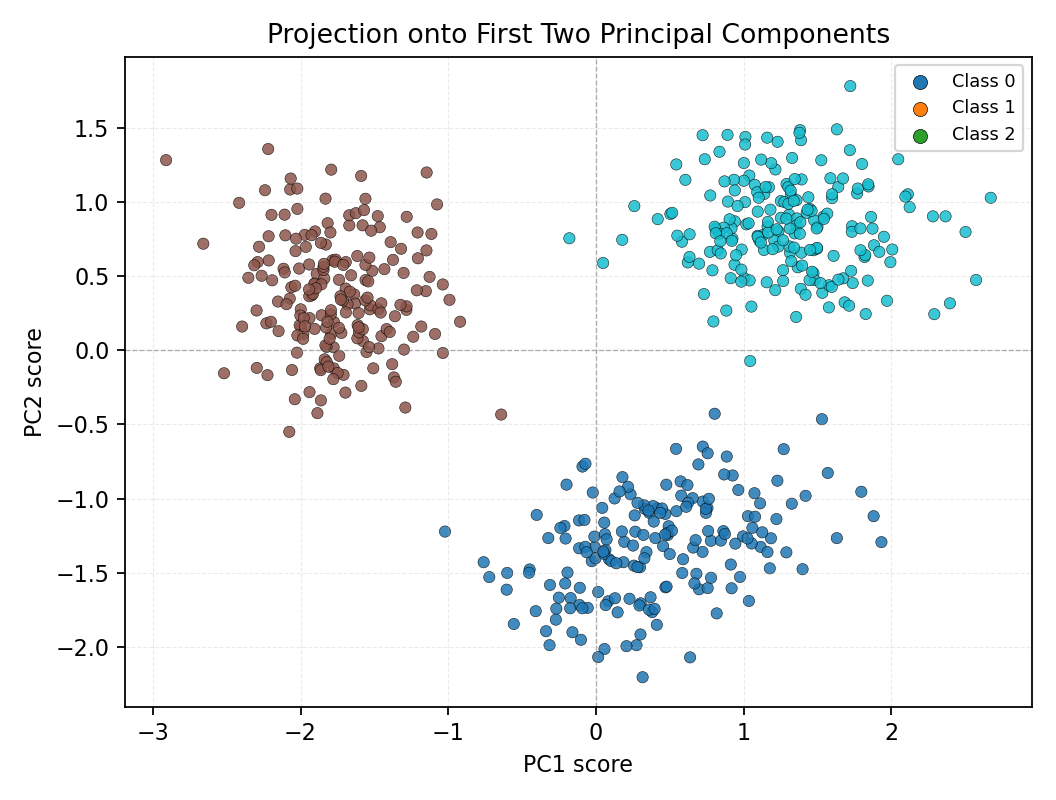
\includegraphics[width=0.82\linewidth]{pca_projection.png}
  \caption{前两个主成分的散点图(按类别着色)}
  \label{fig:pca_projection_cn}
\end{figure}

\begin{figure}[H]
  \centering
  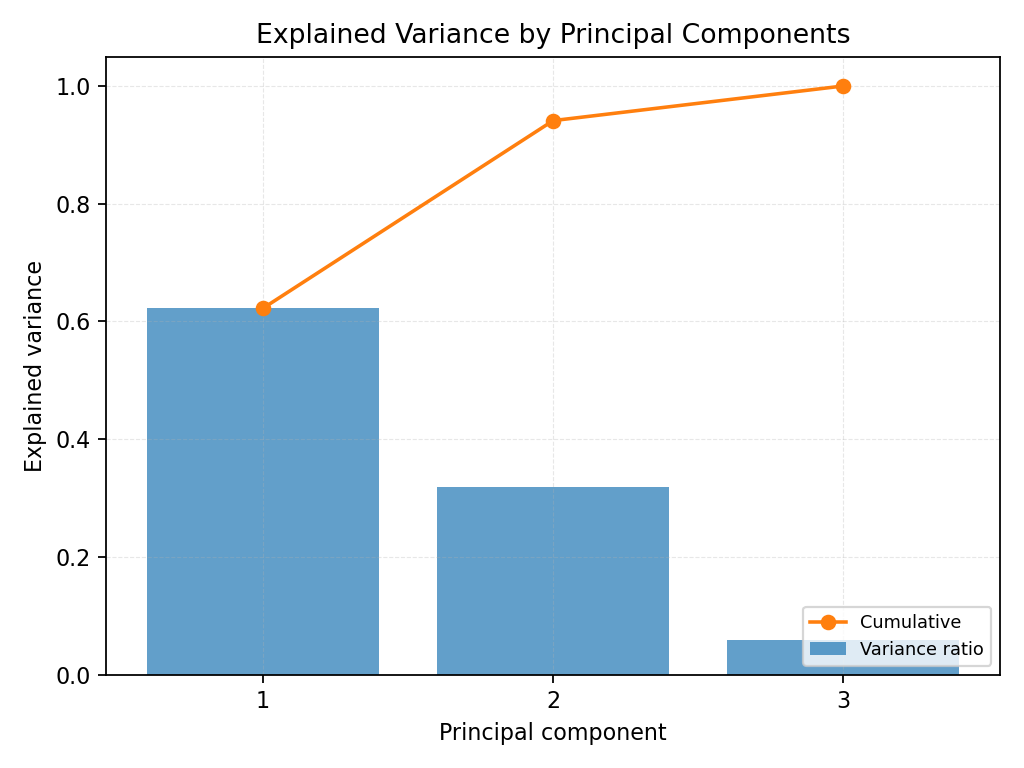
\includegraphics[width=0.8\linewidth]{pca_explained_variance.png}
  \caption{各主成分方差贡献率与累计曲线}
  \label{fig:pca_explained_variance_cn}
\end{figure}

\FloatBarrier
\section{总结}
PCA 通过特征分解或 SVD 提取最大方差方向,实现信息保留与降维之间的权衡。示例展示了主成分散点与方差曲线如何辅助选择保留成分数量。

\end{document}
